\section{Espectrograma}
	\subsection{Construcción de espectrogramas}
	Utilizando la función implementada \texttt{DFTwin}, se procede a calcular el espectro de la vocal \textit{a}, considerando que interesa únicamente, seis períodos de oscilación de la frecuencia fundamental:
	\begin{equation*}
		6 \cdot \frac{1}{f0} = \frac{6}{87} \approx 0.0689~\text{s}
	\end{equation*}
	
	Llevando esto a muestras:
	\begin{equation*}
		S = ceil \left( \frac{6 \cdot fs}{f0} \right) = 552~\text{muestras}
	\end{equation*}
	
	Se sabe que las señales de vocales en general comienzan en la muestra $m = 5000$. Para la resolución espectral, se escoge el mismo largo de la señal, en este caso $N = 552$. Por lo que la función utilizada queda definida como \texttt{DFTwin(a, 552,5000, 552)}. Graficando la magnitud del espectro:
	
	\begin{figure}[H]
		\center
		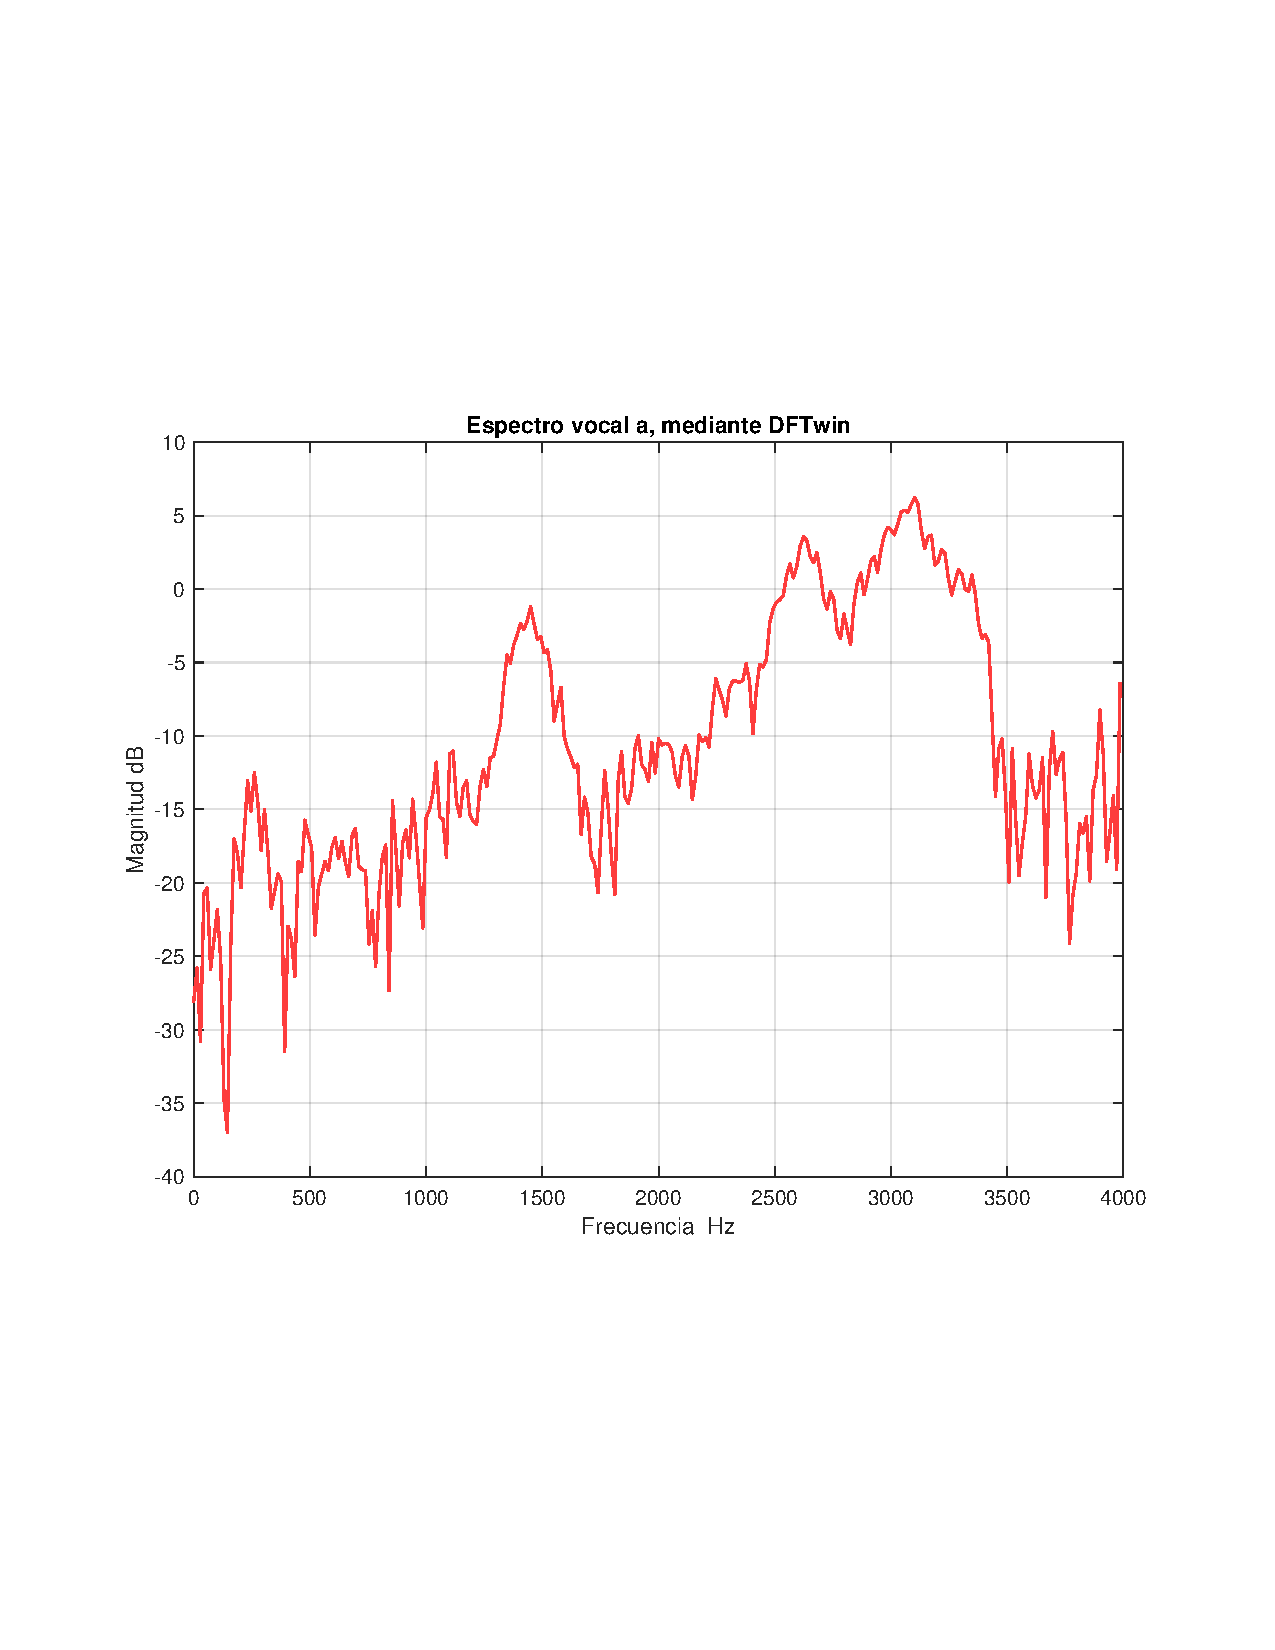
\includegraphics[width=0.6\textwidth,clip, trim = {1.9cm 6.8cm 2.3cm 7cm}]{../plots/a_dftwin.pdf}
		\caption{Espectro de la vocal a, para seis períodos de oscilación}
		\label{fig:fft_6_f0}
	\end{figure}
